\documentclass[12pt,a4paper]{scrartcl}

\usepackage[utf8]{inputenc}
\usepackage[german]{babel}
\usepackage[T1]{fontenc}
\usepackage{amsmath}
\usepackage{amsfonts}
\usepackage{amssymb}
\usepackage{graphicx}
\usepackage{xcolor}
\usepackage{fancyhdr}
%Zeilenabstand von 1.5%
\usepackage{setspace}

\usepackage{float}

\usepackage{bigstrut}
\usepackage{hyperref}
\usepackage{booktabs}

%%Source Code
\usepackage{listings}
\lstset{
  frame=none,
  xleftmargin=2pt,
  stepnumber=1,
  numbers=left,
  numbersep=5pt,
  numberstyle=\ttfamily\tiny\color[gray]{0.3},
  belowcaptionskip=\bigskipamount,
  captionpos=b,
  escapeinside={*'}{'*},
  language=haskell,
  tabsize=2,
  emphstyle={\bf},
  commentstyle=\it,
  stringstyle=\mdseries\rmfamily,
  showspaces=false,
  keywordstyle=\bfseries\rmfamily,
  columns=flexible,
  basicstyle=\small\sffamily,
  showstringspaces=false,
  morecomment=[l]\%,
}

%%%%%%%%%%%%%%%%%%%%%%%
%%Glossar Paket laden%
\usepackage[
nonumberlist, %keine Seitenzahlen anzeigen
acronym,      %ein Abkürzungsverzeichnis erstellen
toc,          %Einträge im Inhaltsverzeichnis
section]      %im Inhaltsverzeichnis auf section-Ebene erscheinen
{glossaries}
%%%%%%%%%%%%%%%%%%%%%%%
\onehalfspacing%Anderthalb Zeilenabstand
%%%%%%%%%%%%%%%%%%%%%%%
\makeglossaries%Glossar
%%%%%%%%%%%%%%%% Titel %%%%%%%%%%%%%%%%%%%%%%%
\title{Entwicklung einer mobilen Webanwendung zur Planung und Unterstützung von Open Spaces.
}
\author{Christoph Hegemann}

%%%%%%%%%%%%%%%%%%%%%%%%%%%%%%%%%%%%%%%%%%%%%%

\begin{document}
\maketitle
\newpage
%\newglossaryentry{ghc}
{
  name=Glasgow Haskell Compiler,
  description={ist der meistgenutzte und fortschrittlichste Haskell Compiler.
    Er ist Open-Source und wird seit seiner ersten lauffähigen Version im Juni 1989 weiterentwickelt\\
    \url{https://www.haskell.org/ghc/}
  }
}
\newglossaryentry{cabal}
{
  name=cabal-install,
  description={ist das de-facto Standard Build und Packaging Tool für Haskell Programme und Bibliotheken\\
    \url{https://www.haskell.org/cabal/}
  }
}
\newglossaryentry{postgresql}
{
  name=PostgreSQL,
  description={ist eine relationale Datenbank die Open-Source entwickelt wird\\
    \url{http://www.postgresql.org/}
  }
}
\newglossaryentry{psc}
{
  name=PureScript Compiler,
  description={ist der PureScript Compiler, der PureScript Source Files in JavaScript übersetzt.\\
    \url{http://www.purescript.org/}
  }
}
\newglossaryentry{react-tools}
{
  name=React Tools,
  description={ist eine Sammlung von Tooling welche bei der Entwicklung von React Komponenten helfen\\
    \url{http://facebook.github.io/react/}
  }
}
\newglossaryentry{pulp}
{
  name=pulp,
  description={ist ein von Bodil Stokke entwickeltes Build-System für PureScript\\
    \url{https://github.com/bodil/pulp}
  }
}
\newglossaryentry{bower}
{
  name=bower,
  description={ist ein Tool für Dependency-Management von Javascript Bibliotheken. Auch die PureScript Community
    verwendet es um Bibliotheken zu verbreiten und verwalten\\
    \url{http://bower.io/}
  }
}
\newglossaryentry{CMS}
{
  name=CMS,
  description={steht für Content-Management-System und beschreibt eine Software zur gemeinschaftlichen
    Erstellung, Bearbeitung und Organisation von Inhalten. In diesem Fall handelt es sich um die Software
    Confluence von Atlassian
  }
}
\newglossaryentry{Event Sourcing}
{
  name=Event Sourcing,
  description={beschreibt ein Vorgehen bei dem alle Zustandveränderungen
    innerhalb eines Systems auf Events abgebildet werden. Dies erlaubt es Vorgänge
    erneut abzuspielen oder die Vergangenheit zu verändern
  }
}
\newglossaryentry{ssh}
{
  name=Secure Shell (ssh),
  description={bezeichnet sowohl ein Netzwerkprotokoll als auch entsprechende Programme, mit deren Hilfe man auf eine sichere Art und Weise eine verschlüsselte Netzwerkverbindung mit einem entfernten Gerät herstellen kann
  }
}
\newglossaryentry{Reactive Programming}
{
  name=Reactive Programming,
  description={beschreibt ein Paradigma, welches sich um Datenflüsse und das Propagieren von Änderungen durch diese dreht.
  Es hat in neuester Zeit an Beliebtheit gewonnen und wird als wichtiger Ansatz gesehen um robuste, skalierbare Systeme zu entwickeln\\
  \url{http://www.reactivemanifesto.org/}
  }
}
\newglossaryentry{React}
{
  name=React,
  description={ist ein von Facebook entwickeltes UI-Framework das ein funktionalen Ansatz für das Erstellen von Oberflächen empfiehlt\\
  \url{http://facebook.github.io/react/}
  }
}
\newglossaryentry{Yesod Framework}
{
  name=Yesod Framework,
  description={ist ein Open-Source Web-Framework, welches in Haskell geschrieben ist und es sich zum Ziel macht Haskells Typsystem zu nutzen,
  um Laufzeitfehler in Compilezeitfehler umzuwandeln.\\
  \url{http://www.yesodweb.com/}
  }
}

%%% Local Variables:
%%% mode: plain-tex
%%% TeX-master: "../Doku"
%%% End:

%\title{Entwicklung einer mobilen Webanwendung zur Planung und Unterstützung von Open Spaces.}
\author{Christoph Hegemann}

%\newcommand{\doublesignature}[2]{%
    \parbox{7cm}{
      \rule{6cm}{1pt}\\
      #1
    }
    \hfill
    \parbox{7cm}{
      \rule{6cm}{1pt}\\
      #2
    }
  }
%%% Local Variables:
%%% mode: latex
%%% TeX-master: "../Doku"
%%% End:

\section{Projektantrag}
\section*{Projektbezeichnung/Auftrag/Teilauftrag}
Entwicklung einer mobilen Webanwendung zur Planung und Unterstützung von Open Spaces.
\subsection*{Ausgangssituation}
Die als Auftraggeber auftretende OPITZ CONSULTING Deutschland GmbH ist ein mittelständisches, wachsendes Unternehmen im Bereich der IT-Beratung und Dienstleistung. Am Hauptsitz in Gummersbach befindet sich neben der Holding Gesellschaft noch der Größte der insgesamt neun Standorte.

\noindent Seit einigen Jahren werden bei Opitz regelmäßig Open Spaces durchgeführt.
Ein Open Space ist eine Veranstaltung, bei der mehrere Personen zusammen kommen, Themen vorschlagen und diese in einer wie auch immer gearteten Weise bearbeiten, besprechen oder erlernen. Ein Open Space verteilt sich hierbei auf mehrere Räume und Timeslots, die zuvor festgelegt werden müssen. Die Themen werden von den Teilnehmern selbst angeboten und die Teilnehmer entscheiden mit ihrer Interessenbekundung an einem oder mehreren Themen, wie sich das Programm gestaltet.
(siehe auch:\footnote{\url{http://en.wikipedia.org/wiki/Open_Space_Technology}})
Falls die Teilnehmer nach Ablauf der Zeit eines Themas weiteres Interesse anmelden kann das Thema ad hoc verlängert und verlegt werden.

\noindent Derzeit verläuft die Planung dieser Open Spaces direkt auf der Veranstaltung mithilfe von Whiteboards oder Flipcharts. Im Nachhinein wird dann zumeist in einem CMS über die Veranstaltungen berichtet und Bilder hochgeladen, wobei dies auf freiwilliger Basis geschieht und zusätzlichen Aufwand bedeutet.

\noindent Dieses sehr statische Planungsvorgehen wird dem dynamischen Charakter von Open Spaces nicht gerecht. Als verteilte Veranstaltung mit ``Realtime''-Aspekt ist für eine sinnvolle Kommunikation ein hohes Maß an Vernetzung unverzichtbar. Das dokumentieren der parallelen und verteilten Vorgänge ist aus der Sicht einer Person aufwendig und das Ergebnis lückenhaft. Eine mobile Webanwendung kann und soll hier Abhilfe schaffen.
\subsection*{Zielsetzung}
Ziel des Projektes ist es, eine erweiterbare Full-Stack-Anwendung zu entwickeln, welche die Durchführung von Open Spaces unterstützt. Der Veranstaltungscharakter legt den Anwendungsfall nahe, eine Instanz dieser Applikation bei Bedarf zu starten und nach der Durchführung der Veranstaltung wieder zu beenden. Hieraus lässt sich die Cloud als geeignete Plattform ableiten. Eine weitere Anforderung an die Anwendung ist ein mobiler Client, der den Teilnehmern eine Sicht auf den aktuellen Zeitplan und die Aufnahme und Verteilung von Bildern und Notizen ermöglicht. Außerdem sollen über den mobilen Client in einem Push-basierten Modell Notifikationen über Änderungen am Zeitplan verteilt werden.
Ein weiteres Ziel ist die Evaluierung von funktionalen Programmiertechniken im Bezug auf ihre Tauglichkeit für die Erstellung von Webapplikationen.
\subsection*{Konsequenzen bei Nichtverwirklichung}
Open Spaces werden weiterhin am Whiteboard geplant und Änderungen am Zeitplan erreichen  Teilnehmer nur dann, wenn diese am zentralen Board nachgetragen werden und die Teilnehmer sich dort regelmäßig über Änderungen informieren. Die Dokumentation des zeitlichen Ablaufs gestaltet sich weiterhin als schwierig.
\section*{Projektumfeld/Rahmenbedingungen}
Um möglichst viele Plattformen (Windows, MacOS, Linux, iOS, Android) und Geräte (Dekstop, Mobile Endgeräte) ansprechen zu können, soll die Entwicklung der Anwendung auf Webtechnologien basieren. Als Versionierungsmodell soll ein Continuous Integration System aufgesetzt werden.
\section*{Projektplanung}
\subsubsection*{Zeitplanung}
\begin{tabular}{l l r}
1. & Planung & 2h \\
2. & Entwurf & 5h \\
\toprule 3. & Implementierung & \\
3.1 & Browser Frontend & 15h \\
3.2 & Backend & 20h \\
3.3 & Mobile Webapp & 5h \\
\toprule 4. & Abschließender Test & 5h \\
5. & Übergabe & 3h \\
6. & Dokumentation & 15h \\
\toprule $\Sigma$ & Summe & 70h
\end{tabular}

\section*{Anzufertigende Dokumente}
\begin{itemize}
\item Projektdokumentation
\item Selbstständigkeitserklärung
\item Screenshots der Anwendung
\item Quellcode
\end{itemize}\section*{Erklärungen}
\subsection*{Erklärung des Prüfungsteilnehmers}
Ich versichere durch meine Unterschrift, dass ich das Projekt und die dazugehörige Dokumentation
selbständig und ohne fremde Hilfe angefertigt und alle Stellen, die ich wörtlich oder annähernd
wörtlich aus Veröffentlichungen entnommen habe, als solche kenntlich gemacht habe. Die Arbeit
hat in dieser Form keiner anderen Prüfungsinstitution vorgelegen.\\[1.5cm]
%\doublesignature{Ort, Datum}{Unterschrift des Prüfungsteilnehmers}
\subsection*{Erklärung des Ausbildungsbetriebes}
Wir versichern, dass das Projekt wie in der Dokumentation dargestellt, in unserem Unternehmen
realisiert worden ist.\\[1.5cm]
%\doublesignature{Ort, Datum}{Unterschrift des Ausbilders}
\section*{Sperrvermerk}
Die vorliegende Abschlussarbeit mit dem Titel ``Entwicklung einer mobilen Webanwendung zur Planung und Unterstützung von Open Spaces'' enthält vertrauliche Daten des Unternehmens OPITZ CONSULTING Deutschland GmbH.
\\[0.5cm]
Die Abschlussarbeit darf nur dem Erst-  und Zweitgutachter sowie  befugten Mitgliedern des
Prüfungsausschusses zugänglich gemacht werden. Eine Veröffentlichung und Vervielfältigung
der Abschlussarbeit ist \- auch in Auszügen \- nicht gestattet.
\\[0.5cm]
Eine Einsichtnahme der Arbeit durch Unbefugte bedarf einer ausdrücklichen Genehmigung des
Verfassers und des Unternehmens OPITZ CONSULTING Deutschland GmbH.
\newpage
\tableofcontents
\newpage
\section{Ausgangssituation}
\subsection{Unternehmensbeschreibung}
Das IT-Beratungshaus OPITZ CONSULTING Deutschland GmbH ist ein wachsendes, mittelständisches Unternehmen im Bereich der IT-Beratung und -Dienstleistung. Am Hauptsitz in Gummersbach befinden sich die Holding-Gesellschaft sowie der Größte der insgesamt neun Standorte. Das Unternehmen ist seit seiner Gründung im Jahr 1990 auf derzeit etwa 450 Mitarbeiter gewachsen. Die 9 Standorte setzen sich aus sieben Standorten in Deutschland, sowie zwei Standorten in Polen zusammen.
\subsection{Projekthintergrund}
Seit einigen Jahren werden bei Opitz regelmäßig Open Spaces durchgeführt.
Ein Open Space ist eine Veranstaltung, bei der mehrere Personen zusammen kommen, Themen vorschlagen und diese in einer wie auch immer gearteten Weise bearbeiten, besprechen oder erlernen. Ein Open Space verteilt sich hierbei auf mehrere Räume und Timeslots, die zuvor festgelegt werden müssen. Die Themen werden von den Teilnehmern selbst angeboten und die Teilnehmer entscheiden mit ihrer Interessenbekundung an einem oder mehreren Themen, wie sich das Programm gestaltet.
(siehe auch:\footnote{\url{http://en.wikipedia.org/wiki/Open_Space_Technology}})
Falls die Teilnehmer nach Ablauf der Zeit eines Themas weiteres Interesse anmelden kann das Thema ad hoc verlängert und verlegt werden.

\noindent Derzeit verläuft die Planung dieser Open Spaces direkt auf der Veranstaltung mithilfe von Whiteboards oder Flipcharts. Im Nachhinein wird dann zumeist in einem CMS über die Veranstaltungen berichtet und Bilder hochgeladen, wobei dies auf freiwilliger Basis geschieht und zusätzlichen Aufwand bedeutet.

\noindent Dieses sehr statische Planungsvorgehen wird dem dynamischen Charakter von Open Spaces nicht gerecht. Als verteilte Veranstaltung mit ``Realtime''-Aspekt ist für eine sinnvolle Kommunikation ein hohes Maß an Vernetzung unverzichtbar. Das dokumentieren der parallelen und verteilten Vorgänge ist aus der Sicht einer Person aufwendig und das Ergebnis lückenhaft. Eine mobile Webanwendung kann und soll hier Abhilfe schaffen.
\section{Projektplanung}
\subsection{IST-Analyse}
\subsection{SOLL-Konzept}
\subsection{Zielsetzung}
\subsection{Infrastrukturelle Rahmenbedingungen}
\subsubsection{Entwicklungsumgebung}
\begin{itemize}
\item OS:Linux
\item IDE:Emacs
\item Browser:Chrome
\item Backend:ghc-mod, stylish-haskell, tern
\end{itemize}
\subsubsection{Laufzeitumgebung}
Das entwickelte Backend soll abschließend auf einem Debian Server laufen. Der Client soll sowohl im Browser auf Desktop Clients als auch in den Browsern der mobilen Clients.
\subsection{Terminplanung}
Das Projekt ist zwischen dem 25.01.2015 und dem 17.04.2015 zu realisieren und umfasst maximal 70 Arbeitsstunden.
\section{Realisierung}
\subsection{Vorgehensweise}
Zu Beginn wurde ein Plan für das grobe Zusammenspiel der beteiligten Komponenten angefertigt. Hiermit wurde die Arbeit in mehrere Schritte und leicht abzugrenzende Komponenten unterteilt. Das Projekt ließ sich damit in Meilensteine aufteilen um strukturiert an das Projekt herangehen zu können.
\subsection{Analyse \& Konzeption}
Bei der Analyse der Anforderungen fallen die Realtime Aspekte auf. Sie sollen mithilfe von Websocketkommunikation und Push-Bases-Updates vom Server umgesetzt werden. Für einen modernen Look und ein intuitives Verhalten auf mobilen Geräten soll die Steuerung Drag and Drop unterstützen.
\subsubsection*{Architektur}
Einen groben Überblick über die spätere ``physikalische Ausprägung'' des Systems soll die Grafik~\ref{fig:architektur} geben.
\begin{figure}[h]
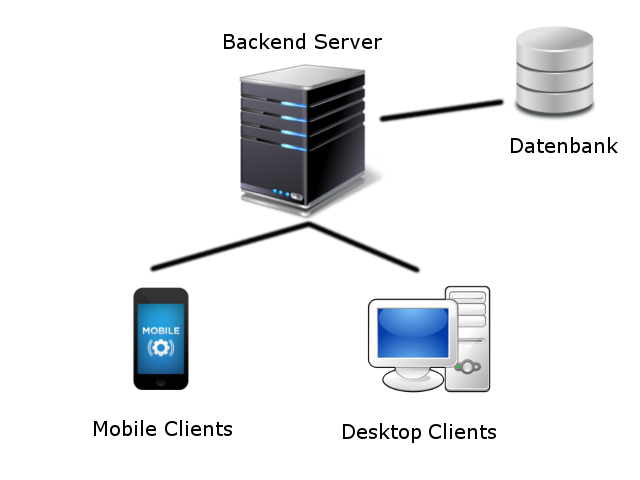
\includegraphics[scale=0.5]{img/Architektur.png}
\caption{Architektur Übersicht\label{fig:architektur}}
\end{figure}
Die Clients (Mobile / Desktop) kommunizieren über WebSockets mit dem Backend-Server. Dieser speichert und liest Daten aus einer Datenbank. Durch die WebSockets ist es dem Backend-Server möglich Änderungen am Datenmodell mittels Push-Benachrichtigungen an die Clients weiterzugeben.
\subsection{Implementierung}
\subsubsection{Browser-Frontend}
Die Implementierung des Browser-Frontends verwendet Technologien, die dem Reactive Pattern zuzuweisen sind.
React.js als UI-Framework von Facebook ist ein stark durch funktionale Ideen inspiriertes Framework. Das Browser Frontend ist modular aufgebaut. Die Kommunikation mittels WebSockets und das Verwalten des Applikationszustandes geschieht im in PureScript implementierten ``Frontend-Backend''. Diese sogenannte Engine nimmt im Unidirectional-Dataflow Modell die Rolle der ``Stores'' ein und erlaubt es das View-Layer beliebig auszutauschen.
\begin{figure}[h]

\includegraphics[scale=0.3]{img/Unidirectional.png}
\caption{Unidirectional Dataflow}
\end{figure}

Die Interaktionen des Benutzers mit dem View-Layer erzeugen dann wiederum Events, die als Streams an die Stores zurückfließen, wo sie interpretiert und verarbeitet werden. Das interpretieren der Events lässt sich dank des deklarativen Stils den PureScript erlaubt, leicht programmieren. Als Beispiel soll der Code dienen, der das Ziehen eines Topics auf das Grid beschreibt.


\begin{lstlisting}
  dragTopic = do
    Right t <- dragStart
    action <- dragOver
    lookup "dragEndTopic" `merge` lookup "dragEndGridTopic"
    return $ action t
\end{lstlisting}

\subsection{Test \& Abnahme}
\subsection{Projektablauf}
\section{Kosten-Nutzen-Betrachtung}
\section{Ausblick}
\section{Fazit}
\section{Glossar}
%Glossar ausgeben
%\printglossary
\section{Anhang}
\subsection{A}
\subsection{B}
\subsection{C}
\end{document}
